\documentclass[]{book}
\usepackage{lmodern}
\usepackage{amssymb,amsmath}
\usepackage{ifxetex,ifluatex}
\usepackage{fixltx2e} % provides \textsubscript
\ifnum 0\ifxetex 1\fi\ifluatex 1\fi=0 % if pdftex
  \usepackage[T1]{fontenc}
  \usepackage[utf8]{inputenc}
\else % if luatex or xelatex
  \ifxetex
    \usepackage{mathspec}
  \else
    \usepackage{fontspec}
  \fi
  \defaultfontfeatures{Ligatures=TeX,Scale=MatchLowercase}
\fi
% use upquote if available, for straight quotes in verbatim environments
\IfFileExists{upquote.sty}{\usepackage{upquote}}{}
% use microtype if available
\IfFileExists{microtype.sty}{%
\usepackage{microtype}
\UseMicrotypeSet[protrusion]{basicmath} % disable protrusion for tt fonts
}{}
\usepackage[margin=1in]{geometry}
\usepackage{hyperref}
\hypersetup{unicode=true,
            pdftitle={BIO 4022. Análisis y manipulación de datos en R},
            pdfauthor={Derek Corcoran},
            pdfborder={0 0 0},
            breaklinks=true}
\urlstyle{same}  % don't use monospace font for urls
\usepackage{natbib}
\bibliographystyle{apalike}
\usepackage{color}
\usepackage{fancyvrb}
\newcommand{\VerbBar}{|}
\newcommand{\VERB}{\Verb[commandchars=\\\{\}]}
\DefineVerbatimEnvironment{Highlighting}{Verbatim}{commandchars=\\\{\}}
% Add ',fontsize=\small' for more characters per line
\usepackage{framed}
\definecolor{shadecolor}{RGB}{248,248,248}
\newenvironment{Shaded}{\begin{snugshade}}{\end{snugshade}}
\newcommand{\AlertTok}[1]{\textcolor[rgb]{0.94,0.16,0.16}{#1}}
\newcommand{\AnnotationTok}[1]{\textcolor[rgb]{0.56,0.35,0.01}{\textbf{\textit{#1}}}}
\newcommand{\AttributeTok}[1]{\textcolor[rgb]{0.77,0.63,0.00}{#1}}
\newcommand{\BaseNTok}[1]{\textcolor[rgb]{0.00,0.00,0.81}{#1}}
\newcommand{\BuiltInTok}[1]{#1}
\newcommand{\CharTok}[1]{\textcolor[rgb]{0.31,0.60,0.02}{#1}}
\newcommand{\CommentTok}[1]{\textcolor[rgb]{0.56,0.35,0.01}{\textit{#1}}}
\newcommand{\CommentVarTok}[1]{\textcolor[rgb]{0.56,0.35,0.01}{\textbf{\textit{#1}}}}
\newcommand{\ConstantTok}[1]{\textcolor[rgb]{0.00,0.00,0.00}{#1}}
\newcommand{\ControlFlowTok}[1]{\textcolor[rgb]{0.13,0.29,0.53}{\textbf{#1}}}
\newcommand{\DataTypeTok}[1]{\textcolor[rgb]{0.13,0.29,0.53}{#1}}
\newcommand{\DecValTok}[1]{\textcolor[rgb]{0.00,0.00,0.81}{#1}}
\newcommand{\DocumentationTok}[1]{\textcolor[rgb]{0.56,0.35,0.01}{\textbf{\textit{#1}}}}
\newcommand{\ErrorTok}[1]{\textcolor[rgb]{0.64,0.00,0.00}{\textbf{#1}}}
\newcommand{\ExtensionTok}[1]{#1}
\newcommand{\FloatTok}[1]{\textcolor[rgb]{0.00,0.00,0.81}{#1}}
\newcommand{\FunctionTok}[1]{\textcolor[rgb]{0.00,0.00,0.00}{#1}}
\newcommand{\ImportTok}[1]{#1}
\newcommand{\InformationTok}[1]{\textcolor[rgb]{0.56,0.35,0.01}{\textbf{\textit{#1}}}}
\newcommand{\KeywordTok}[1]{\textcolor[rgb]{0.13,0.29,0.53}{\textbf{#1}}}
\newcommand{\NormalTok}[1]{#1}
\newcommand{\OperatorTok}[1]{\textcolor[rgb]{0.81,0.36,0.00}{\textbf{#1}}}
\newcommand{\OtherTok}[1]{\textcolor[rgb]{0.56,0.35,0.01}{#1}}
\newcommand{\PreprocessorTok}[1]{\textcolor[rgb]{0.56,0.35,0.01}{\textit{#1}}}
\newcommand{\RegionMarkerTok}[1]{#1}
\newcommand{\SpecialCharTok}[1]{\textcolor[rgb]{0.00,0.00,0.00}{#1}}
\newcommand{\SpecialStringTok}[1]{\textcolor[rgb]{0.31,0.60,0.02}{#1}}
\newcommand{\StringTok}[1]{\textcolor[rgb]{0.31,0.60,0.02}{#1}}
\newcommand{\VariableTok}[1]{\textcolor[rgb]{0.00,0.00,0.00}{#1}}
\newcommand{\VerbatimStringTok}[1]{\textcolor[rgb]{0.31,0.60,0.02}{#1}}
\newcommand{\WarningTok}[1]{\textcolor[rgb]{0.56,0.35,0.01}{\textbf{\textit{#1}}}}
\usepackage{longtable,booktabs}
\usepackage{graphicx,grffile}
\makeatletter
\def\maxwidth{\ifdim\Gin@nat@width>\linewidth\linewidth\else\Gin@nat@width\fi}
\def\maxheight{\ifdim\Gin@nat@height>\textheight\textheight\else\Gin@nat@height\fi}
\makeatother
% Scale images if necessary, so that they will not overflow the page
% margins by default, and it is still possible to overwrite the defaults
% using explicit options in \includegraphics[width, height, ...]{}
\setkeys{Gin}{width=\maxwidth,height=\maxheight,keepaspectratio}
\IfFileExists{parskip.sty}{%
\usepackage{parskip}
}{% else
\setlength{\parindent}{0pt}
\setlength{\parskip}{6pt plus 2pt minus 1pt}
}
\setlength{\emergencystretch}{3em}  % prevent overfull lines
\providecommand{\tightlist}{%
  \setlength{\itemsep}{0pt}\setlength{\parskip}{0pt}}
\setcounter{secnumdepth}{5}
% Redefines (sub)paragraphs to behave more like sections
\ifx\paragraph\undefined\else
\let\oldparagraph\paragraph
\renewcommand{\paragraph}[1]{\oldparagraph{#1}\mbox{}}
\fi
\ifx\subparagraph\undefined\else
\let\oldsubparagraph\subparagraph
\renewcommand{\subparagraph}[1]{\oldsubparagraph{#1}\mbox{}}
\fi

%%% Use protect on footnotes to avoid problems with footnotes in titles
\let\rmarkdownfootnote\footnote%
\def\footnote{\protect\rmarkdownfootnote}

%%% Change title format to be more compact
\usepackage{titling}

% Create subtitle command for use in maketitle
\newcommand{\subtitle}[1]{
  \posttitle{
    \begin{center}\large#1\end{center}
    }
}

\setlength{\droptitle}{-2em}

  \title{BIO 4022. Análisis y manipulación de datos en R}
    \pretitle{\vspace{\droptitle}\centering\huge}
  \posttitle{\par}
    \author{Derek Corcoran}
    \preauthor{\centering\large\emph}
  \postauthor{\par}
      \predate{\centering\large\emph}
  \postdate{\par}
    \date{2018-08-02}

\usepackage{booktabs}

\begin{document}
\maketitle

{
\setcounter{tocdepth}{1}
\tableofcontents
}
\hypertarget{parte-i}{%
\chapter*{Parte I}\label{parte-i}}
\addcontentsline{toc}{chapter}{Parte I}

\hypertarget{requerimientos}{%
\chapter{Requerimientos}\label{requerimientos}}

La última versión de RStudio y R \citep{R-base}, también se requiere de
los paquetes \emph{pacman}, \emph{tidyverse} y \emph{tinytex}.

Si no han usado R o RStudio, pueden ver un video de como instalar ambos
programas, asi como los paquetes más necesarios para este curso, que son
\emph{pacman}, \emph{rmarkdown}, \emph{tidyverse} y \emph{tinytex} en el
siguiente \href{https://youtu.be/RtkCAKXsVbw}{link}.

El código para la instalación de esos paquetes es el siguiente

\begin{Shaded}
\begin{Highlighting}[]
\KeywordTok{install.packages}\NormalTok{(}\StringTok{"pacman"}\NormalTok{, }\StringTok{"rmarldown"}\NormalTok{, }\StringTok{"tidyverse"}\NormalTok{, }\StringTok{"tinytex"}\NormalTok{)}
\end{Highlighting}
\end{Shaded}

Si necesitan ayuda para la instalación contactarse con elinstructor del
curso.

\hypertarget{si-nunca-has-usado-r-antes}{%
\section{Si nunca has usado R antes}\label{si-nunca-has-usado-r-antes}}

Si nunca han usado \texttt{R} antes de este curso, porfavor installar el
paquete \href{http://swirlstats.com/students.html}{Swirl}
\citep{Kross2017} y realizar los primeros 7 modulos del programa \emph{R
Programming: The basics of programming in R} que incluye:

\begin{itemize}
\tightlist
\item
  Basic Building Blocks
\item
  Workspace and Files
\item
  Sequences of Numbers
\item
  Vectors
\item
  Missing Values
\item
  Subsetting Vectors
\item
  Matrices and Data Frames
\end{itemize}

Pueden ver un video explicativo de como usar swirl en el siguiente
\href{https://youtu.be/w6L7Ye18yPE}{Video}

\hypertarget{descripcion}{%
\section{Descripción}\label{descripcion}}

Este curso está enfocado en entregar los principios de investigación
reproducible en R, con énfasis en la recopilación y/o lectura de datos
de forma reproducible y automatizada. Para esto se trabajará con bases
de datos complejos, las cuales deberán ser transformadas y organizadas
para optimizar su análisis. Se generarán documentos reproducibles
integrando en un documento código, bibliografía, exploración y análisis
de datos. Se culminará el curso con la generación de un manuscrito,
presentación y/o documento interactivo reproducible.

\hypertarget{objetivos}{%
\section{Objetivos}\label{objetivos}}

\begin{enumerate}
\def\labelenumi{\arabic{enumi}.}
\item
  Conocer y entender el concepto de Investigación reproducible como un
  forma y filosofía de investigación que permite que las investigaciones
  sean más ordenadas y replicables, desde la toma de datos hasta la
  escritura de resultados.
\item
  Conocer y aplicar el concepto de pipeline, el cual permite generar una
  modularidad desde la toma de datos hasta la escritura de resultados,
  donde la corrección independiente de un paso tiene un efecto cascada
  sobre el resultado final.
\item
  Aprender buenas prácticas de recolección y estandarización de bases de
  datos, con la finalidad de optimizar el análisis de datos y la
  revisión de estas por pares.
\item
  Realizar análisis críticos de la naturaleza de los datos al realizar
  análisis exploratorios, que permitirán determinar la mejor forma de
  comprobar hipótesis asociadas a estas bases de datos.
\end{enumerate}

\hypertarget{contenidos}{%
\section{Contenidos}\label{contenidos}}

\begin{itemize}
\item
  Capítulo \ref{tidydata} \emph{Tidy Data}: En este capítulo,
  aprenderemos de como optimizar una de base de datos, limpieza y
  transformación de bases de datos, que es una base de datos
  \emph{tidy}, y como manipular estas bases de datos con el paquete
  \emph{dplyr} \citep{R-dplyr}
\item
  Capitulo \ref{reproducible} \emph{Investigación reproducible}:
  entenderemos el como generar un documento que combine códigos de
  \texttt{R} y texto para generar documentos reporducibles utilizando el
  paquete \emph{rmarkdown} \citep{Allaire2018}, además veremos como al
  usar RStudio podemos guardar nuestro proyecto en un repositorio de
  github.
\item
  Capitulo \ref{tidyverso} \emph{El tidyverso}, el concepto de pipeline.
  Limpieza de datos complejos
\end{itemize}

\begin{enumerate}
\def\labelenumi{\arabic{enumi}.}
\setcounter{enumi}{4}
\item
  Visualización de datos, visualizar datos vs.~visualizar modelos.
  Insertar gráficos con leyenda en un documento Rmd
\item
  Creación de funciones propias y loops. Generación de funciones propias
  en R y loops
\item
  Escritura de manuscritos en R, transformación de documentos Rmd en un
  manuscrito
\item
  Presentaciones en R y generar documentos interactivos. Transformación
  de datos en una presentación o en una Shiny app. Realizar una
  presentación o aplicación en R.
\end{enumerate}

\hypertarget{metodologia}{%
\section{Metodología}\label{metodologia}}

Todas las clases serán prácticas y estarán divididas en dos partes: I.
Clases de principios y herramientas, donde se presentarán los principios
de investigación reproducible y tidy data, junto con las herramientas
actuales más utilizadas, y II. Clases aplicadas donde se trabajará con
datos propios para desarrollar un documento reproducible. A los
estudiantes que no cuenten con datos propios, se les será proporcionado
un set de datos o se simularán dependiendo del caso.

Además se deberán generar informes y presentaciones siguiendo los
principios de investigación reproducible, usando datos propios o
entregados. Se realizará un informe final, en el cual se espera un
trabajo

\hypertarget{evaluacion}{%
\section{Evaluación}\label{evaluacion}}

\begin{itemize}
\tightlist
\item
  Evaluación 1: Informe exploratorio de base de datos 25\%
\item
  Evaluación 2: Presentación 25\%
\item
  Evaluación 3: Informe final 50\%
\end{itemize}

\hypertarget{objetivo-del-curso}{%
\section{Objetivo del curso}\label{objetivo-del-curso}}

Aprender los principios de investigación reproducible y tidy data a
través del aprendizaje de programación y uso de R. Los principios de
este curso están explicados en los siguientes libros gratuitos.

\begin{itemize}
\tightlist
\item
  Gandrud, Christopher. Reproducible Research with R and R Studio. CRC
  Press, 2013. Available for free in the following
  \href{https://englianhu.files.wordpress.com/2016/01/reproducible-research-with-r-and-studio-2nd-edition.pdf}{link}
\item
  Stodden, Victoria, Friedrich Leisch, and Roger D. Peng, eds.
  Implementing reproducible research. CRC Press, 2014. Available for
  free in the following
  \href{http://web.stanford.edu/~vcs/papers/ijclp-STODDEN-2009.pdf}{link}
\end{itemize}

\hypertarget{bibliografia}{%
\section{Bibliografía}\label{bibliografia}}

\hypertarget{tidydata}{%
\chapter{Tidy Data y manipulación de datos}\label{tidydata}}

En este capítulo explicaremos que es una base de datos \emph{tidy}
\citep{wickham2014tidy} y aprenderemos a usar funciones del paquete
\emph{dplyr} \citep{R-dplyr} para manipular datos.

Recuerda que este libro es un apoyo para el curso BIO4022, puedes seguir
la clase de este curso en este
\href{https://derek-corcoran-barrios.github.io/Clase1/Clase1TidyData}{link},
y en cuanto el video de la clase este disponible encontrarás un link
aca.

\hypertarget{tidy-data}{%
\section{Tidy data}\label{tidy-data}}

Una base de datos tidy es una base de datos en la cuál (modificado de
\citep{leek2015elements}):

\begin{itemize}
\tightlist
\item
  Cada varaible que midas debiera estar en una columna.
\item
  Cada observación distinta de esa variable debiera estar en una fila
  diferente.
\end{itemize}

\hypertarget{dplyr}{%
\section{dplyr}\label{dplyr}}

El paquete \emph{dplyr} es definido por sus autores como una gramática
para la manipulación de datos. De este modo sus funciones son conocidas
como verbos. Un resumen útil de muchas de estas funciones se encuentra
en este
\href{https://www.rstudio.com/wp-content/uploads/2015/02/data-wrangling-cheatsheet.pdf}{link}.

Este paquete tiene un gran número de verbos y sería difícil ver todos en
una clase, en este capítulo nos enfocaremos en sus funciones más
utilizadas, las cuales son:

\begin{itemize}
\tightlist
\item
  \emph{group\_by} (agrupa datos)
\item
  \emph{summarize} (resume datos agrupados)
\item
  \emph{filter} (Encuentra filas con ciertas condiciones)
\item
  \emph{select} junto a \emph{starts\_with}, \emph{ends\_with} o
  \emph{contains}
\item
  \emph{mutate} (Genera variables nuevas)
\item
  \emph{\%\textgreater{}\%} pipeline
\end{itemize}

\hypertarget{reproducible}{%
\chapter{Investigación reproducible}\label{reproducible}}

Here is a review of existing methods.

\hypertarget{tidyverso}{%
\chapter{El Tidyverso}\label{tidyverso}}

We describe our methods in this chapter.

\hypertarget{visualizacion}{%
\chapter{Visualización de datos}\label{visualizacion}}

En este capítulo aprenderemos a usar el paquete \emph{ggplot2}
\citep{Wickhamggplot}, parte del paquete \emph{tidyverse}
\citep{Wickhamtidyverse}.

\hypertarget{el-esqueleto}{%
\section{El esqueleto}\label{el-esqueleto}}

El esqueleto de una visualización usando \emph{ggplot2} es la siguiente

\begin{Shaded}
\begin{Highlighting}[]
\KeywordTok{ggplot}\NormalTok{(data.frame, }\KeywordTok{aes}\NormalTok{(nombres de columna)) }\OperatorTok{+}\StringTok{ }\KeywordTok{geom_algo}\NormalTok{(argumentos, }\KeywordTok{aes}\NormalTok{(columnas)) }\OperatorTok{+}\StringTok{ }\KeywordTok{theme_algo}\NormalTok{()}
\end{Highlighting}
\end{Shaded}

Como ejemplo para discutir usaremos el siguiente código que genera la
figura \ref{fig:ejemplo1-ggplot}:

\begin{Shaded}
\begin{Highlighting}[]
\KeywordTok{library}\NormalTok{(tidyverse)}
\KeywordTok{data}\NormalTok{(}\StringTok{"diamonds"}\NormalTok{)}
\KeywordTok{ggplot}\NormalTok{(diamonds, }\KeywordTok{aes}\NormalTok{(}\DataTypeTok{x =}\NormalTok{ carat, }\DataTypeTok{y=}\NormalTok{price)) }\OperatorTok{+}\StringTok{ }\KeywordTok{geom_point}\NormalTok{(}\KeywordTok{aes}\NormalTok{(}\DataTypeTok{color =}\NormalTok{ cut)) }\OperatorTok{+}\StringTok{ }\KeywordTok{theme_classic}\NormalTok{()}
\end{Highlighting}
\end{Shaded}

\begin{figure}

{\centering 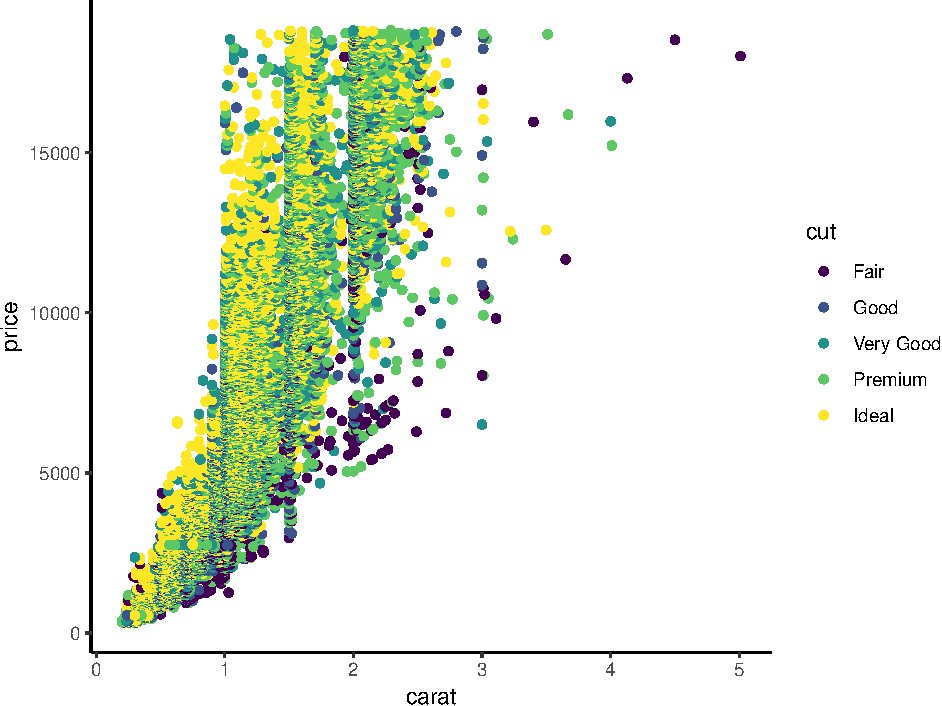
\includegraphics[width=0.8\linewidth]{Libro_files/figure-latex/ejemplo1-ggplot-1} 

}

\caption{Gráfico en el cual gráficamos los quilates de diamantes versus su precio, con el corte del diamante representado por el color}\label{fig:ejemplo1-ggplot}
\end{figure}

En este caso general, lo primero que ponemos después de ggplot es el
data.frame desde el cuál graficaremos algo, en el ejemplo de la figura
\ref{fig:ejemplo1-ggplot} usamos la base de datos \emph{diamonds} del
paquete \emph{ggplot2} \citep{Wickhamggplot}. Luego dentro de
\texttt{aes} ponemos las columnas que graficaremos como \emph{x} y/o
\emph{y}, en nuestro ejemplo dentro de aes ponemos como eje \emph{x} los
kilates de los diamantes (caret) y como \emph{y} el precio de los mismos
(price). La necesidad de poner \texttt{aes} en ggplot2 (algo que no
había sido necesario cuando usamos \emph{dplyr} o \emph{tidyr}) es que
ggplot2 es el paquete mas antiguo del \emph{tidyverse}.

\hypertarget{geom_algo}{%
\section{geom\_algo}\label{geom_algo}}

Luego de especificar una base de datos, esto viene seguido de un
\texttt{geom\_algo}, esto nos indicará que tipo de gráfico usaremos,
estos pueden ser combinados como veremos en ejemplos futuros

\hypertarget{una-variable-categorica-una-continua}{%
\subsection{Una variable categórica una
continua}\label{una-variable-categorica-una-continua}}

Primero veremos algunos de los \emph{geom} que podemos utilizar con una
variable categórica y una continua

\hypertarget{geom_boxplot}{%
\subsubsection{geom\_boxplot}\label{geom_boxplot}}

En la figura \ref{fig:boxplot}, generado a partir del código a
continuacón con la base de datos iris presente en \texttt{R}
\citep{anderson1935irises}.

\begin{Shaded}
\begin{Highlighting}[]
\KeywordTok{data}\NormalTok{(}\StringTok{"iris"}\NormalTok{)}
\KeywordTok{ggplot}\NormalTok{(iris, }\KeywordTok{aes}\NormalTok{(}\DataTypeTok{x =}\NormalTok{ Species, }\DataTypeTok{y =}\NormalTok{ Sepal.Length)) }\OperatorTok{+}\StringTok{ }\KeywordTok{geom_boxplot}\NormalTok{()}
\end{Highlighting}
\end{Shaded}

\begin{figure}

{\centering 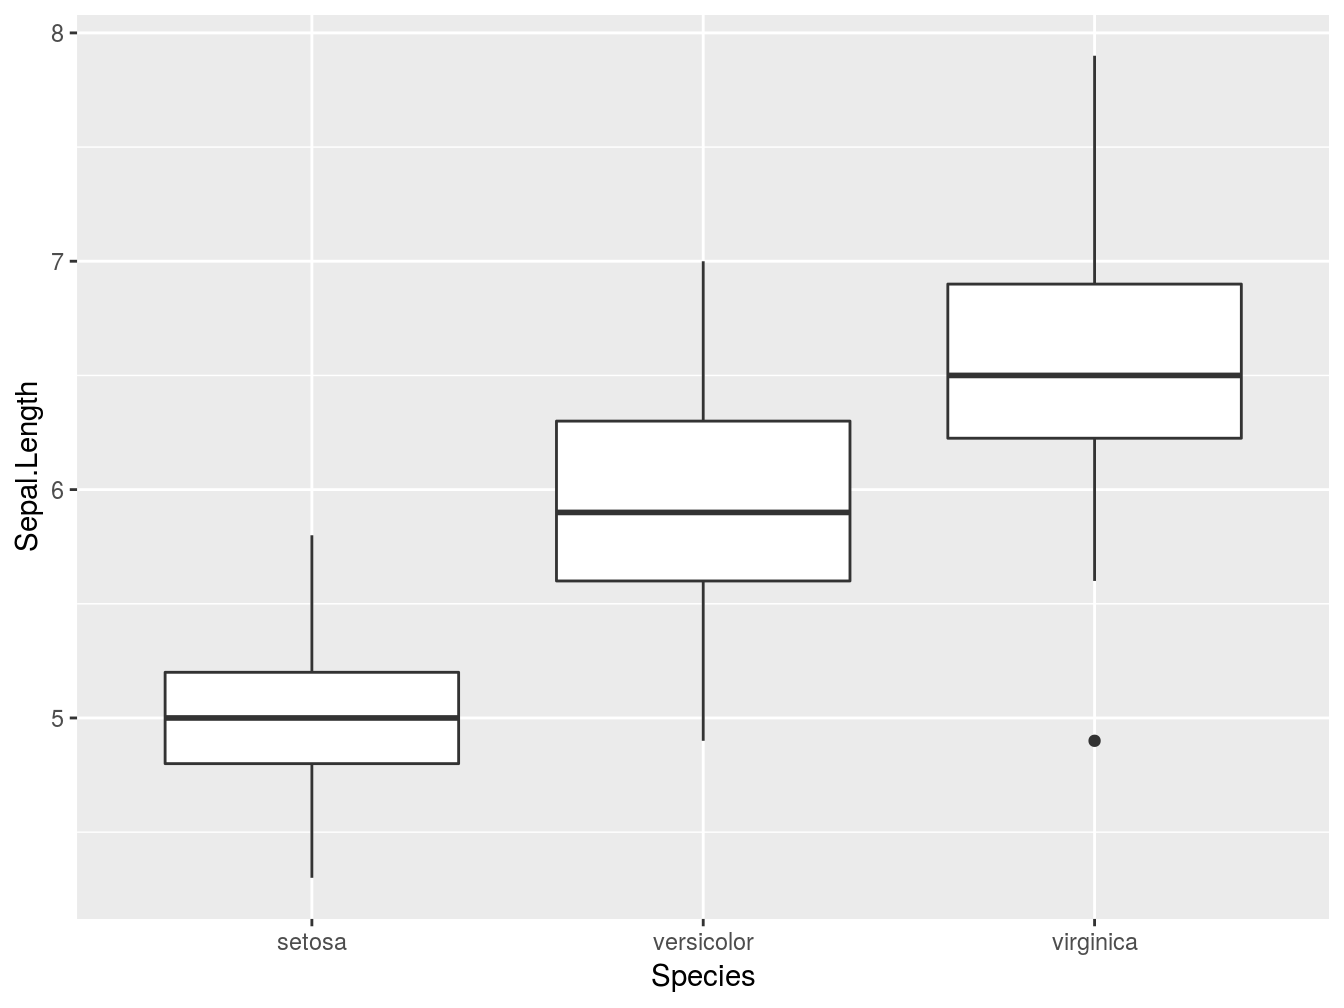
\includegraphics[width=0.8\linewidth]{Libro_files/figure-latex/boxplot-1} 

}

\caption{Boxplot que representa los largos del sépalo de tres especies del género Iris}\label{fig:boxplot}
\end{figure}

Los boxplots muestran una linea gruesa central (la mediana), una caja,
que delimita el primer y tercer cuartil, y los bigotes, los cuales se
extienden hasta los valores extremos. A menos que estos esten por sobre
1.5 veces la distance entre el primer y tercer cuartil, en cuyo caso se
consideran outlyers, y estos son representados por puntos. En la figura
\ref{fig:boxplot}, solo \emph{Iris virginica} presenta un outlayer en
cuanto a las medidas del largo del sepalo.

Los boxplots, como todos los gráficos pueden ser personalizados usando
otros argumentos, los cuales son detallados en la sección
\ref{argumentos}, pero en los ejemplos que mostraremos en esta sección
los iremos introduciendo de a poco. Si quisieramos por ejemplo que el
color de las cajas del \emph{boxplot} fuera deacuerdo a la especie,
cambiamos el llenado (\textbf{fill}) de la caja, como vemos en el
siguiente ejemplo y figura \ref{fig:boxplot2}

\begin{Shaded}
\begin{Highlighting}[]
\KeywordTok{ggplot}\NormalTok{(iris, }\KeywordTok{aes}\NormalTok{(}\DataTypeTok{x =}\NormalTok{ Species, }\DataTypeTok{y =}\NormalTok{ Sepal.Length)) }\OperatorTok{+}\StringTok{ }\KeywordTok{geom_boxplot}\NormalTok{(}\KeywordTok{aes}\NormalTok{(}\DataTypeTok{fill =}\NormalTok{ Species))}
\end{Highlighting}
\end{Shaded}

\begin{figure}

{\centering 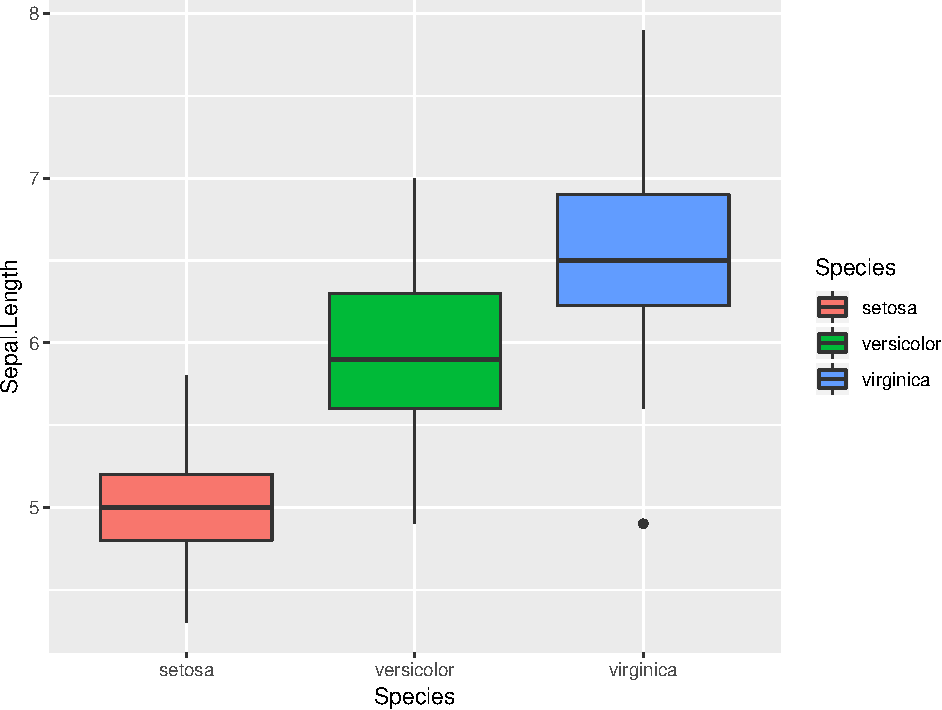
\includegraphics[width=0.8\linewidth]{Libro_files/figure-latex/boxplot2-1} 

}

\caption{Boxplot que representa los largos del sépalo de tres especies del género Iris, en este caso el color de la caja representa la especie}\label{fig:boxplot2}
\end{figure}

Dos cosas a notar en este ejemplo, por un lado la leyenda se genera de
forma automática, y por otro lado, vemos que es necesario poner
\emph{Species} dentro de \texttt{aes}, esto es debido a que Species es
una columna y como se explicó al principio de este capítulo, todas las
columnas deben ser incuidas dentro de la función \texttt{aes} para poder
ser referenciadas.

\hypertarget{geom_jitter}{%
\subsubsection{geom\_jitter}\label{geom_jitter}}

\begin{Shaded}
\begin{Highlighting}[]
\KeywordTok{ggplot}\NormalTok{(iris, }\KeywordTok{aes}\NormalTok{(}\DataTypeTok{x =}\NormalTok{ Species, }\DataTypeTok{y =}\NormalTok{ Sepal.Length)) }\OperatorTok{+}\StringTok{ }\KeywordTok{geom_jitter}\NormalTok{(}\KeywordTok{aes}\NormalTok{(}\DataTypeTok{color =}\NormalTok{ Species))}
\end{Highlighting}
\end{Shaded}

\begin{figure}

{\centering 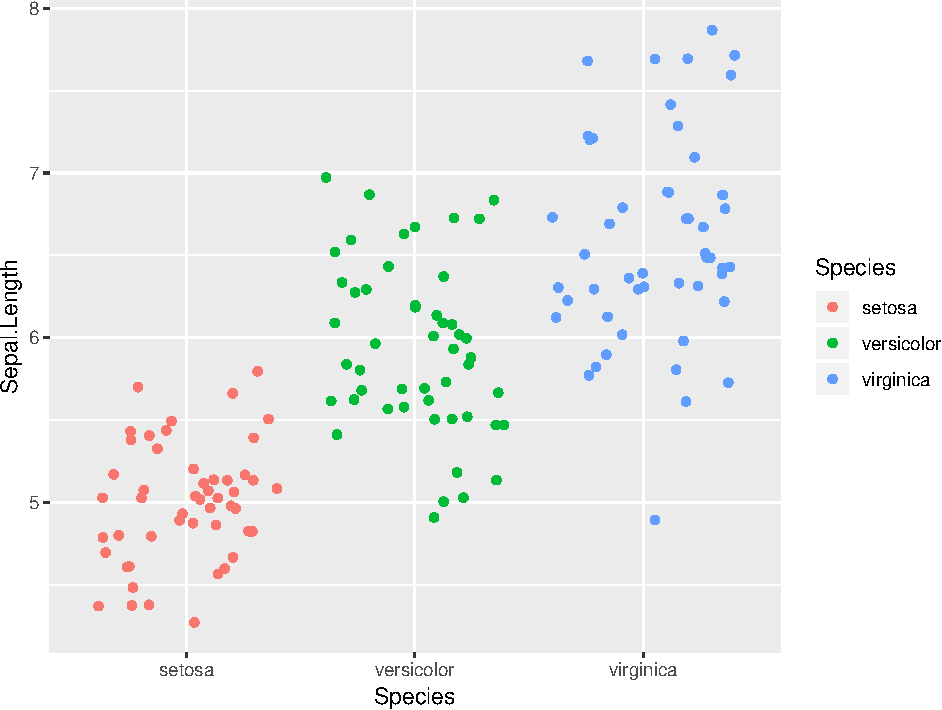
\includegraphics[width=0.8\linewidth]{Libro_files/figure-latex/jitter-1} 

}

\caption{Boxplot que representa los largos del sépalo de tres especies del género Iris, en este caso el color de la caja representa la especie}\label{fig:jitter}
\end{figure}

\hypertarget{argumentos}{%
\section{Argumentos}\label{argumentos}}

\hypertarget{modelos}{%
\chapter{Modelos en R}\label{modelos}}

We have finished a nice book.

\hypertarget{loops}{%
\chapter{Loops (purrr) y bibliografía (rticles)}\label{loops}}

\hypertarget{presentacion}{%
\chapter{Presentaciones en R}\label{presentacion}}

\bibliography{book.bib,packages.bib}


\end{document}
